\section{Results}
\label{sec:results}

%Performance Evaluation, Results, Discussion}

%\textit{owners: Evan: graphs, All: interpretation (2.75 pages)}

\subsection{CX Performance using C and MPI} %%on Single Node}
  \label{sxn:results1}


   
%%  \vspace*{0.1in}

      In Table~\ref{tab:single_node}, we show the benefits of various
      optimizations described in
      Sec.~\ref{sxn:single_node_opt}. 
      %%%%
      %%%%
      %%%%
      %to the performance of \textsc{MultiplyGramian} and \textsc{Multiply} on each compute node. 
      %%
      %%
      %The test matrix $\mathcal{A}$ has {\it{m}} = 1.95M, {\it{n}} = 128K,
      %{\it{s}} = 0.004, and {\it{nnz}} = 10$^9$. The parameter
      %{\it{k}} = 32. 
      As far as single-node performance is concerned, we started with a parallelized implementation  
      without any of the described optimizations. %%, and measured the performance (in terms of time taken). 
      We first implemented the multi-core synchronization scheme, wherein a single copy of the
      output matrix is maintained, %% across all the threads (for the matrix multiplication).
      which resulted in a speedup of 6.5X, primarily due to
      the reduction in the amount of data traffic between 
      main memory and caches. 
      %%last-level cache and main memory (there was around 19X measured reduction in traffic). 
      We then implemented our cache blocking scheme, which led to a
      further  2.4X speedup (overall 15.6X).
%%      primarily targeted towards ensuring that the output of the matrix multiplication resides in the caches (since it is
%      accessed and updated frequently). This led to a further 2.4X reduction in run-time, for an overall speedup of around 15.6X.
      We then implemented our SIMD code that sped it up by a further
      2.6X, for an overall speedup of 39.7X. Although the 
      SIMD width is 4, 
        %%($\mathcal{S}$ = 4),
        there are overheads of address
        computation, stores, and not all computations (e.g. QR) were
        vectorized.
        %%(QR code is still scalar).



%%     Once the memory traffic was optimized for, we implemented our
%%     SIMD code by vectorizing the element-row multiplication-add
%%     operations (described in detail in Sec.~\ref{sxn:single_node_opt}). 
%%     The resultant code sped up by a further 2.6X, for an overall
%%     speedup of 39.7X. Although the effective SIMD width
%% ($\mathcal{S}$ = 4), there are overheads of address computation,
%% stores, and not all computations were vectorized (QR code is still %% scalar).



        As far as the multi-node performance is concerned, 
 on the Amazon EC2 cluster, with 30 nodes (960-cores in total), and
 the 1 TB dataset as input, it
 took 151 seconds to perform CX computation (including time to load
 the data into main memory). 
%% and 92 seconds to load the data.
 %read in data into main memory. 
 As compared to the Scala code on the same platform (details in
 next sec.), we achieve a speedup of 21X.
 %%(in terms of compute time) and 6.7X (data load  + compute time.)
%
 % We did a head-to-head comparison of C code with the Scala node, 
 %%%%implementation on a single node, 
 %and measured a performance gap of around 21X.
 This performance gap can be attributed to the careful cache
 optimizations of maintaining single copy of the output matrix shared
 across threads, bandwidth friendly access of matrices and vector
 computation using SIMD units.

 Some of these optimizations can be implemented in Spark, such as arranging the
 order of memory accesses to make efficient use of memory. %%of the memory bus.
 However, other optimizations such as sharing the output matrix between threads
 and use of SIMD intrinsics fall outside the Spark programming model, and would
 require piercing the abstractions provided by Spark and JVM.
 %to more directly access and manipulate the hardware.
 Thus there is a tradeoff between optimizing performance 
 and ease of implementation, %% and efficient global scheduling, 
 available by expressing programs in the Spark programming model.

 
  \begin{table}
  \begin{center}
  \begin{tabular}{ |c|c| } 
  \hline
  Single Node Optimization & Overall Speedup\\
  \hline
  Original Implementation & 1.0  \\
  Multi-Core Synchronization & 6.5 \\
  Cache Blocking & 15.6 \\
  SIMD & 39.7 \\
  \hline

  \end{tabular}
  \end{center}
  \caption{Single node opt. to CX C implementation and
  subsequent speedup  each additional optimization provides.}
  \label{tab:single_node}
  \end{table}
 



  \subsection{CX Spark Performance} %% on Spark} across Multiple Nodes}
%  \textcolor{red}{Mike R, Jatin: we need a narrative here}

  \subsubsection{CX Spark Phases}
  Our implementations of CX and PCA share the \textsc{RandomizedSVD} subroutine, which accounts for the bulk of the runtime and all of the distributed computations.
  The execution of \textsc{RandomizedSVD} proceeds in four distributed phases listed below, along with a small amount of additional local computation.
  \begin{enumerate}
      \item \textbf{Load Matrix Metadata}
         The dimensions of the matrix are read from the distributed filesystem to the driver.
      \item \textbf{Load Matrix}
         A distributed read is performed to load the matrix entries into an in-memory cached
         RDD containing one entry per row of the matrix.
      \item \textbf{Power Iterations}
          The \textsc{MultiplyGramian} loop (lines 2-5) of
         \textsc{RandomizedSVD} is run to compute an approx. $Q$
         of the dominant right singular subspace.
       \item \textbf{Finalization (Post-Processing)}
           Right multiplication by $Q$ (line 7) of \textsc{RandomizedSVD} to compute $C$.
  \end{enumerate}

  \subsubsection{Empirical Results}

    \begin{figure} [h!btp]
    \begin{centering}
    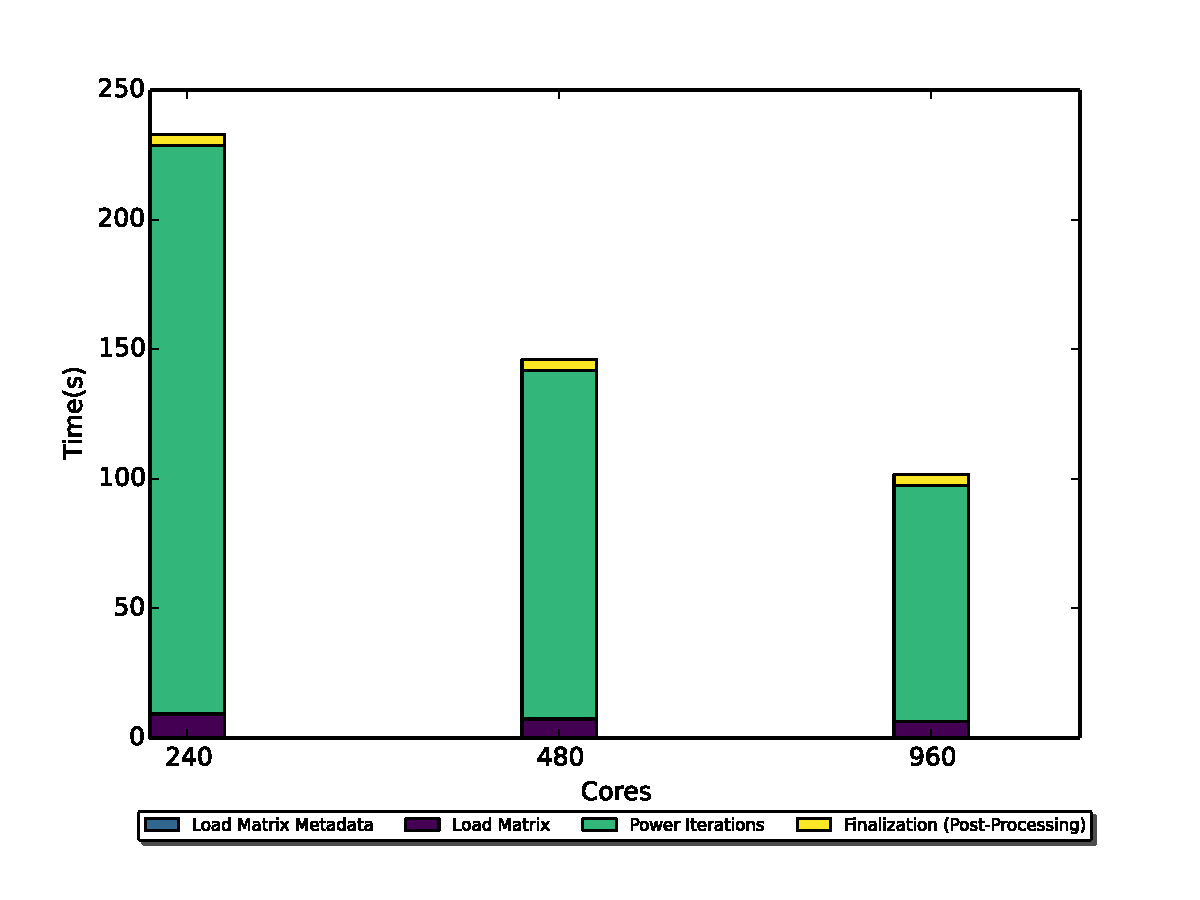
\includegraphics[scale=0.4]{images/CX_Strong_Scaling_New_Colors_Axes_Rank_32_Partitions_default.pdf}
    \end{centering}
    \caption{ Strong scaling for the 4 phases of CX on an XC40 for 100GB dataset at $k=32$ and default partitioning as concurrency is increased.} 
    \label{fig:xc40scaling}
    \end{figure} 

Fig.~\ref{fig:xc40scaling} shows how the distributed Spark portion of our code scales. %% as we add additional processors.  
We considered 240, 480, and 960 cores.  An additional doubling (to 1920 cores) would be ineffective as there are only 1654 partitions, 
so many cores would remain unused.  
%%%In addition, with fewer partitions per core there are fewer opportunities for load balancing and speculative reexecution of slow tasks.
%%
When we go from 240 to 480 cores, we achieve a speedup of 1.6x: %% from doubling the cores: 
233 seconds versus 146 seconds.  However, as the number of partitions per core drops 
below two, and the amount of computation-per-core relative to communication overhead drops, 
the scaling slows down (as expected).  
This results in a lower speedup of 1.4x (146 seconds versus 102
seconds) from 480 to 960 cores.
%%when we double the core count to 960.

  \subsection{CX Performance across Multiple Platforms}
  \label{sect:h2h}
    
    \begin{figure} [h!btp]
    \begin{centering}
    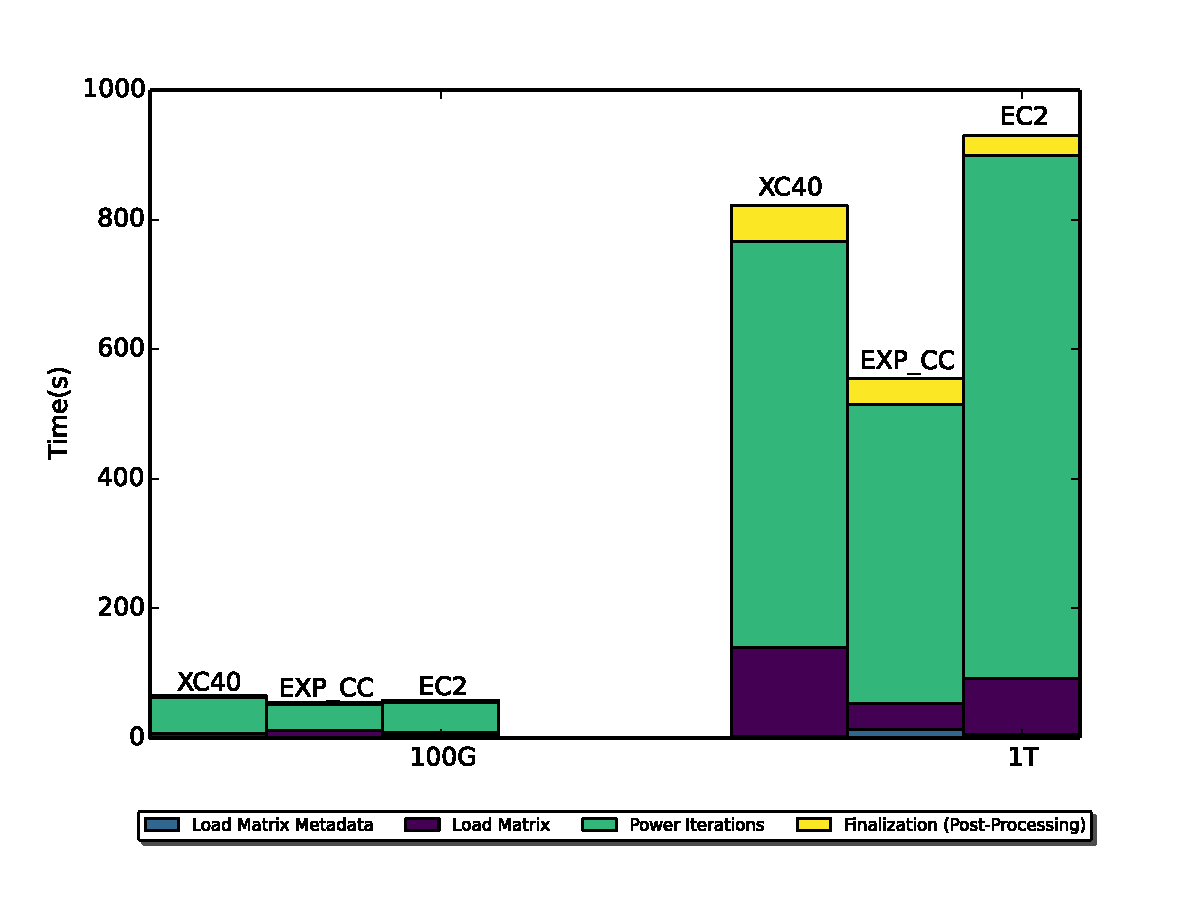
\includegraphics[scale=0.4]{images/CX_Size_Scaling_New_Colors_Axes_Rank_16_Partitions_default.pdf}
    \end{centering}
    \caption{ Run times for the various stages of computation for CX for two different dataset sizes for the three platforms using $k=16$ and default partitioning for the given platform} 
    \label{fig:h2hrank16} 
    \end{figure}

    
      \begin{figure} [H]
    \begin{centering}
    \includegraphics[scale=0.4]{images/CX_Size_Scaling_Rank_32_Partitions_default.pdf}
    \end{centering}
    \caption{ Run times for the various stages of computation for CX for two different dataset sizes for the three platforms using $k=32$ and default partitioning for the given platform}
    \label{fig:h2hrank32} 
    \end{figure}
    
    \begin{table*}
    \begin{center}
    \begin{tabular}{| l | c | c | c | c | c | c | c |}
    \toprule
    \textbf{Platform} & \textbf{Rank} & \textbf{Total} & \textbf{Load} & \textbf{Time Per} & \textbf{Average} & \textbf{Average} & \textbf{Average} \\
                               & & \textbf{Runtime} & \textbf{Time} & \textbf{Iteration} & \textbf{Local} & \textbf{Aggregation} & \textbf{Network} \\
                               & & & & & \textbf{Task} & \textbf{Task} & \textbf{Wait} \\
    \midrule
    Amazon EC2 \texttt{r3.8xlarge} & 16 & 24.0 min & 1.53 min & 2.69 min & 4.4 sec & 27.1 sec & 21.7 sec \\
    \midrule
    Cray XC40 & 16 & 23.1 min& 2.32 min & 2.09 min &  3.5 sec & 6.8 sec & 1.1 sec \\
    \midrule
    Experimental Cray cluster & 16 & 15.2 min & 0.88 min & 1.54 min &  2.8 sec & 9.9 sec & 2.7 sec \\
    \midrule
    Amazon EC2 \texttt{r3.8xlarge} & 32 & 52.6 min& 1.57 min & 5.42 min &  8.7 sec & 60.1 sec & 48.7 sec \\
    \midrule
    Cray XC40 & 32 & 41.2 min & 2.28 min & 4.01 min &  7.5 sec & 25.0 sec & 15.4 sec \\
    \midrule
   Experimental Cray cluster & 32 & 35.8 min & 0.81 min & 3.82 min &  6.8 sec & 27.9 sec & 15.5 sec \\
   \bottomrule
    \end{tabular}
    \end{center}
    \caption{Total runtime for the 1 TB dataset, broken down into load time and per-iteration time. The per-iteration time is further broken down into the average time for each task of the local stage and each task of the aggregation stage.  We also show the average amount of time spent waiting for a network fetch, to illustrate the impact of the interconnect.}
    \label{tab:h2hres1TB}
    \end{table*}
    
Table~\ref{tab:h2hres1TB} shows the total runtime of CX for the 1 TB dataset on our three platforms.  The distributed Spark portion of the computation is also depicted visually in Figures~\ref{fig:h2hrank16} ($k=16$) and~\ref{fig:h2hrank32} ($k=32$).  All three platforms were able to successfully process the 1 TB dataset at $k=16$ in under 25 minutes.  As the table and figures illustrate, most of the variation between the platforms occurred during the \texttt{MultiplyGramian} iterations.  Table~\ref{tab:hwspecs} shows the specifications of the three platforms. In this section, we explore how these difference relate to the performance of the matrix iterations.

Spark divides each iteration into two stages.  The first \emph{local} stage computes each row's contribution, sums the local results (the rows computed by the same worker node), and records these locally-aggregated results.  The second \emph{aggregation} stage combines all of the workers' locally-aggregated results using a tree-structured reduction.  Most of the variation between platforms occurs during the aggregation phase, where data from remote worker nodes is fetched and combined.  In Spark, all inter-node data exchange occurs via \emph{shuffle operations}.  In a shuffle, workers with data to send write the data to their local scratch space.  Once all data has been written, workers with data to retrieve from remote nodes request that data from the sender's block manager, which in turns retrieves if from the senders local scratch space, and sends it over the interconnect to the receiving node.

Examining our three platforms (Table~\ref{tab:hwspecs}), we notice two key hardware differences that impact shuffle operations:
\begin{itemize}
\item First, both the EC2 nodes and the experimental Cray cluster nodes have fast SSD storage local to the compute nodes that they can use to store Spark's shuffle data.  
The Cray{\textsuperscript{\tiny\textregistered}}~XC40{\textsuperscript{\tiny\texttrademark}} system's~\cite{alverson2012cray,craycascadesc12} nodes, on the other hand, have no local persistent storage devices.  Thus we must emulate local storage with a remote Lustre filesystem.  The impacts of this can be somewhat mitigated, however, by leaving sufficient memory to store some of the data in a local RAM disk, and/or to locally cache some of the remote writes to Lustre.\footnote{This is an ideal usage of caching, since Spark assumes the scratch space is only locally accessible; thus we are guaranteed that the only node that reads a scratch file will be the same node that wrote it.}
\item Second, the Cray XC40 and the experimental Cray cluster both communicate over the HPC-optimized Cray Aries 
interconnect~\cite{alverson2012cray,craycascadesc12}, while the EC2 nodes use 10 Gigabit Ethernet.
\end{itemize}  

   \begin{figure} [H]
    \begin{centering}
    \includegraphics[scale=0.4]{images/boxplot_read_write_task_new_Rank_16_1T_default_partitions.pdf}
    \end{centering}
    \caption{A box and whisker plot of the distribution of local (write) and aggregation (read) task times on our three platforms for the 1TB dataset with $k=16$.  The boxes represent the 25th through 75th percentiles, and the lines in the middle of the boxes represent the medians.  The whiskers are set at 1.5 box widths outside the boxes, and the crosses are outliers (results outside the whiskers).  Note that each iteration has 4800 write tasks and just 68 read tasks.}
    \label{fig:rwtaskdist} 
    \end{figure}

We can see the impact of differing interconnect capabilities in the Average Network Wait column in Table~\ref{tab:h2hres1TB}.   These lower average network wait times explain why the two Cray platforms outperform the EC2 instance (with the experimental cluster achieving a speedup of roughly 1.5x over EC2).  

The XC40 is still slightly slower than the experimental Cray cluster, however, in particular at $k=16$.
Part of this difference is due to the slower matrix load phase on the XC40.  On EC2 and the experimental
Cray cluster, the input matrix is stored in SSDs on the nodes running the Spark executors.  Spark is 
aware of the location of the HDFS blocks, and attempts to schedule tasks on the same nodes as their 
input.  The XC40, however, lacks SSDs on its compute nodes, so the input matrix is instead stored on a 
parallel Lustre file system.  The increased IO latency slows the input tasks. The rest of the difference in 
performance can be understood by looking at the distribution of local (write) task times in the box and 
whiskers plot in Figure~\ref{fig:rwtaskdist}.  The local/write tasks are much more numerous than the 
aggregation/read tasks (4800 vs 68 per iteration), thus they have a more significant impact on 
performance. We see that the XC40 write tasks had a similar median time to the experimental cluster's 
write tasks, but a much wider distribution.  The large tail of slower "straggler" tasks is the result of some shuffle data going to the remote Lustre file system rather than being cached locally. We enabled Spark's optional speculative re-execution (\texttt{spark.speculation}) for the XC40 runs, and saw that some of these tasks were successfully speculatively executed on alternate nodes with more available OS cache, and in some case finished earlier.  This eliminated many of the straggler tasks and brought our performance closer to the experimental Cray cluster, but still did not match it (the results in Figures~\ref{fig:h2hrank16} and~\ref{fig:h2hrank32} and Table~\ref{tab:h2hres1TB} include this configuration optimization).  We discuss future directions for improving the performance on Spark on HPC systems in Section~\ref{sect:lessons}.


  
%  \subsection{Timing and Accuracy comparison of RSVD, CX, and truncated SVD}

% Because the RSVD allows us to explicitly control its accuracy by tuning the number of iterations $q$,
% the reconstruction error of the low-rank approximation obtained from the RSVD
% algorithm is expected to be somewhat lower than that of truncated SVD
% approximation. Similarly, CX decompositions have the advantage of
% interpretability, but come at the cost of an increased number of operations on
% top of the RSVD and an additional loss in approximation accuracy. 

%  In Figures~\ref{fig:timing-accuracy-8} and~\ref{fig:timing-accuracy-16}, we observe the timing vs accuracy tradeoffs of the RSVD and CX algorithms
%  as applied to the 100G MSI dataset for two settings of the rank parameter, $k=8$ and $k=16$. The exact SVD was computed in this case using the
%  Spark bindings of the popular ARPACK eigenproblem library~\cite{ArpackUserGuide}. The RSVD algorithm used two power iterations, and we used the output of the RSVD algorithm to generate
%  both the column CX decomposition defined in Algorithm~\ref{alg:cx} and a related `row CX' decomposition that comes from applying Algorithm~\ref{alg:cx}
%  to $A^T.$ As explained in more detail in the next section, both of these CX decompositions are of interest, as they identify important pixels and ions.
%
%  For both rank parameters, we observe the behavior predicted by the theory for the RSVD decomposition: the approximation error is only slightly greater than that of the 
%  truncated SVD approximation. We also observe that there is only a slight speed advantage to using the RSVD; this is likely attributable to the fact that the input matrix
%  is truly low-rank (more than 70\% of the Frobenius norm of the matrix is already captured by the rank-8 decomposition), so the iterative ARPACK SVD algorithm converges 
%  quite fast.
%
%  The CX decompositions require significantly more time to compute than the truncated SVD and RSVD decompositions. This is due to the need to compute the projection of $A$ onto
%  the columns $C$ after $C$ is constructed according to Algorithm~\ref{alg:cx}. We also note that for the MSI dataset, row-based CX decompositions are more 
%  accurate and less expensive to construct than column-based CX decompositions. 
%
%  \begin{figure}[h!btp]
%    \begin{centering}
%      \includegraphics[scale=0.4]{images/timing-accuracy-8}
%      \end{centering}
%      \caption{The Frobenius norm approximation errors and timings for three runs of the RSVD and CX approximations relative to those of the truncated SVD for a target rank of $8$ on the 100G MSI dataset.}
%    \label{fig:timing-accuracy-8}
%  \end{figure}
%
%  \begin{figure}[h!btp]
%    \begin{centering}
%      \includegraphics[scale=0.4]{images/timing-accuracy-16}
%      \end{centering}
%      \caption{The Frobenius norm approximation errors and timings for three runs of the RSVD and CX approximations relative to those of the truncated SVD for a target rank of $16$ on the 100G MSI dataset.}
%    \label{fig:timing-accuracy-16}
%  \end{figure}

  \subsection{Science Results}
  
  \begin{figure}[h!bt]
    \centering
    \includegraphics[width=.9\columnwidth]{images/cx_ions.pdf}
      \caption{Normalized leverage scores (sampling probabilities) for $m/z$ marginalized over $\tau$.
        Three narrow regions of $m/z$ account for $59.3\%$ of the total probability mass.}
      \label{fig:cx_ions}
  \end{figure} 

  The rows and columns of our data matrix $A$ correspond to pixels and $(\tau, m/z)$ values of ions, respectively. 
  We compute the CX decompositions of both $A$ and $A^T$ in order to identify important ions in addition to important pixels.
   
  In Figure~\ref{fig:cx_ions}, we present the distribution of the normalized
  ion leverage scores marginalized over $\tau$. That is, each score corresponds
  to an ion with $m/z$ value shown in the $x$-axis. Leverage scores of ions in
  three narrow regions have significantly larger magnitude than the rest. This
  indicates that these ions are more informative and should be kept as basis
  for reconstruction.  Encouragingly, several other ions with significant
  leverage scores are chemically related to the ions with highest leverage
  scores.  For example, the ion with an $m/z$ value of 453.0983 has the second
  highest leverage score among the CX results.  Also identified as having
  significant leverage scores are ions at $m/z$ values of 439.0819, 423.0832,
  and 471.1276, which correspond to neutral losses of $\rm{CH_2}$,
  $\rm{CH_2O}$, and a neutral ``gain'' of $\rm{H_2O}$ from the 453.0983 ion.
  These relationships indicate that this set of ions, all identified by CX as
  having significant leverage scores, are chemically related.  That fact
  indicates that these ions may share a common biological origin, despite
  having distinct spatial distributions in the plant tissue sample.
  

  \subsection{Improving Spark on HPC Systems}
  \label{sect:lessons}
  
  The differences in performance between the Cray{\textsuperscript{\tiny\textregistered}}~XC40{\textsuperscript{\tiny\texttrademark}} system~\cite{alverson2012cray,craycascadesc12} and the experimental Cray cluster point to optimizations to Spark that could improve its performance on HPC-style architectures.  The two platforms have very similar configurations, with the primary difference being the lack of local persistent storage on the XC40 nodes.  As described in Section~\ref{sect:h2h}, this forces some of Spark's local scratch space to be allocated on the remote Lustre file system, rather than in local storage.  To mitigate this, and keep more of the scratch data local, we propose the following future work:
\begin{itemize}
\item Spark is currently inefficient in cleaning up its local scratch space.  In particular, shuffle data is not immediately cleaned up after a shuffle completes.  This makes fault recovery more efficient, but results in higher storage requirements for scratch space.  If clean up was more efficient, it would be more feasible to fit all of the scratch data in a local RAM disk and not rely on Lustre at all.
\item Spark does not currently allow you to configure primary and backup scratch directories.  Instead you list all scratch directories in a single list, and it distributes data in a round round fashion between them as long as space is available.  You can bias it towards one storage device (e.g., RAM disk vs. Lustre) by listing multiple directories on the preferred device.  Ideally, though, we would like to use a RAM disk (or other local storage) exclusively unless and until it fills, and only switch to Lustre directories if necessary.
\item Spark does not allow you to specify that a scratch directory is globally accessible.  Thus non-cached data is stored to the remote Lustre directory by the sender, and then later retrieved by the sender and sent to the receiver.  This wastes a step, since the receiver could easily fetch the data directly from Lustre (or any other global file system).
\item Alternatively, a push model of communication (as opposed to the current pull model) might be possible - however this would have implications for reliability and handling of very large data sets.\footnote{Storing the shuffle data to a large persistent block storage device, and only sending it as needed, allows Spark to easily shuffle more data than could fit in the remote buffers.  In a push-based model, extra logic and synchronization would be necessary to ensure that the remote buffers do not overflow.}
\end{itemize}


